\documentclass{beamer}
\usepackage{graphicx}
\usepackage{amsmath, amsthm, amsfonts, amssymb, mathrsfs, mathtools, caption, subcaption}
\usepackage{textcomp} % straigth apos
\usepackage{tikz}
\usepackage{verbatim}
\usepackage{tikzit}
\usepackage{listings}
\usepackage[ruled,vlined, linesnumbered]{algorithm2e}
\usepackage{algorithmic,float}
\usepackage[
  % audience=short
  audience=long
]{beameraudience}

\input{graphs.tikzstyles}
\usetikzlibrary{decorations.pathreplacing}

\usefonttheme{serif}

\theoremstyle{definition}

\setbeamercovered{invisible}

\setbeamertemplate{theorems}[numbered]
\setbeamertemplate{lemma}[numbered]
\newtheorem{remark}{Remark}

\usetheme{Madrid}
\useoutertheme{tree} % Alternatively: miniframes, infolines, split
\useinnertheme{circles}


\setbeamertemplate{headline}
{%
  \leavevmode%
  \begin{beamercolorbox}[wd=.5\paperwidth,ht=2.5ex,dp=1.125ex]{section in head/foot}%
    \hbox to .5\paperwidth{\hfil\insertsectionhead\hfil}
  \end{beamercolorbox}%
  \begin{beamercolorbox}[wd=.5\paperwidth,ht=2.5ex,dp=1.125ex]{subsection in head/foot}%
    \hbox to .5\paperwidth{\hfil\insertsubsectionhead\hfil}
  \end{beamercolorbox}%
}

\setbeamertemplate{section in toc}{%
  \inserttocsectionnumber.~\inserttocsection}
\setbeamercolor{section in toc}{fg=black}
\setbeamercolor{subsection in toc}{fg=structure}
\setbeamertemplate{subsection in toc}{%
  \hspace{1.2em}{\tiny\inserttocsectionnumber.\inserttocsubsectionnumber}~\small\inserttocsubsection\par}

% \setbeamertemplate{bibliography item}{\insertbiblabel.~\insertbibitem}

\definecolor{maincolor}{RGB}{78, 145, 94}

\usecolortheme[named=maincolor]{structure}

\title[End-of-studies internship]{Verification in Isabelle/HOL of Hopcroft’s algorithm for minimizing DFAs including runtime analysis}
\date{\today}
\author[V. Trélat]{Vincent Trélat}
\institute[TUM]{Technical University of Munich\\Chair for Logic and Verification}

\newcommand{\prompt}[1]{vtrelat@home:\raisebox{0.5ex}{\texttildelow}\$ #1}

% Outline:
% - Life in Munich
% - TUM and the Chair for Logic and Verification
%     - Teaching
%     - Research : Isabelle
% - Introduce the internship
%     - The algorithm
%     - Verification of correctness
%     - Verification of time complexity


\begin{document}

\begin{frame}
\begin{figure}
\centering
\hfill

\includegraphics[height=9mm]{../img/logoartem.png}\hfill

\includegraphics[height=9mm]{../img/logoTUM.png}\hfill

\includegraphics[height=9mm]{../img/logoisabelle.png}\hfill
\hfill
\end{figure}
\titlepage
\end{frame}

\begin{frame}
    \frametitle{Outline}
    \tableofcontents
\end{frame}

\section{Living in Munich}
\subsection{The city}

\begin{frame}
    \only<1>{
    \begin{figure}
        \centering
        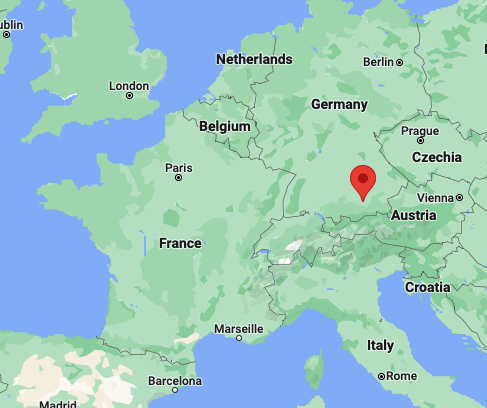
\includegraphics[width=0.5\textwidth]{img/map.png}
        \caption{Location of Munich}
    \end{figure}
    }
    \only<2>{
    \begin{figure}
        \centering
        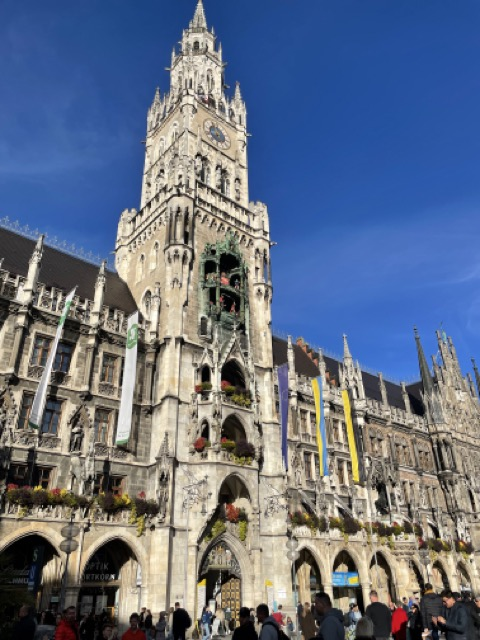
\includegraphics[height=4cm]{img/munich1.jpeg}
        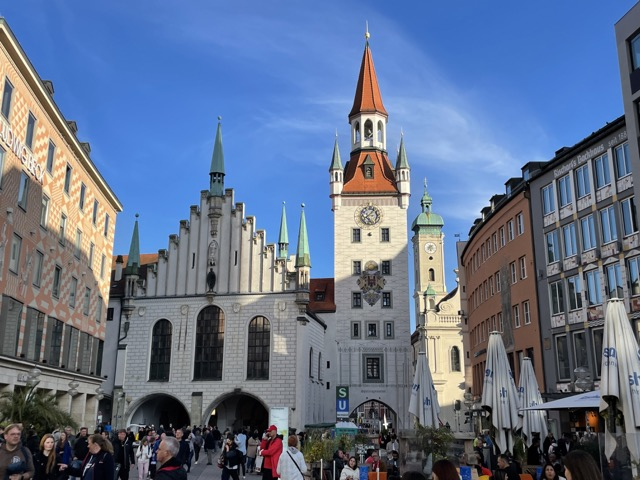
\includegraphics[height=4cm]{img/munich2.jpeg}
        \vfill
        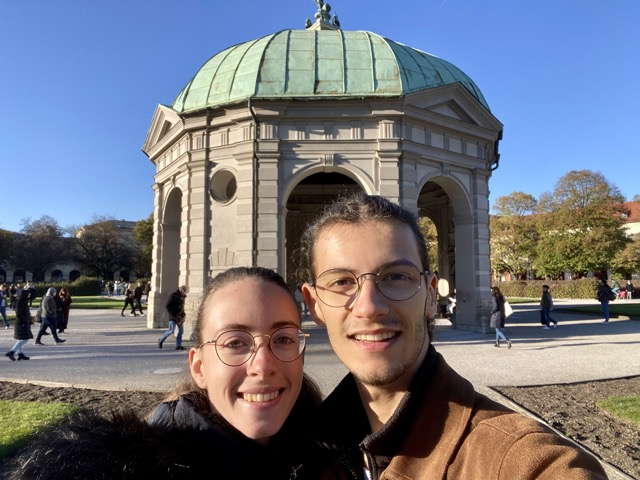
\includegraphics[height=3cm]{img/munich3.jpeg}
        \caption{Some photos of Munich}
    \end{figure}
    }
    \onslide<3->{
    \begin{figure}
        \centering
        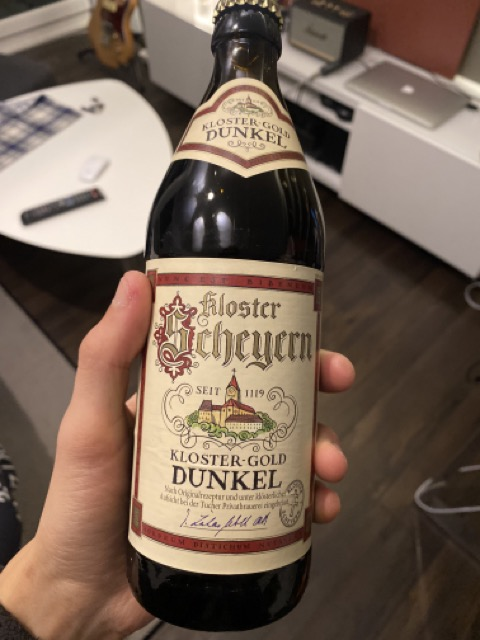
\includegraphics[height=3cm]{img/beer0.jpeg}
        \onslide<4->{
\includegraphics[height=3.2cm]{img/beer1.jpeg}}
        \onslide<5->{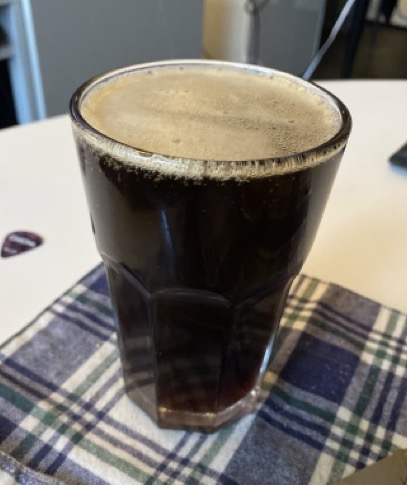
\includegraphics[height=3.2cm]{img/beer2.jpeg}}
        \onslide<6->{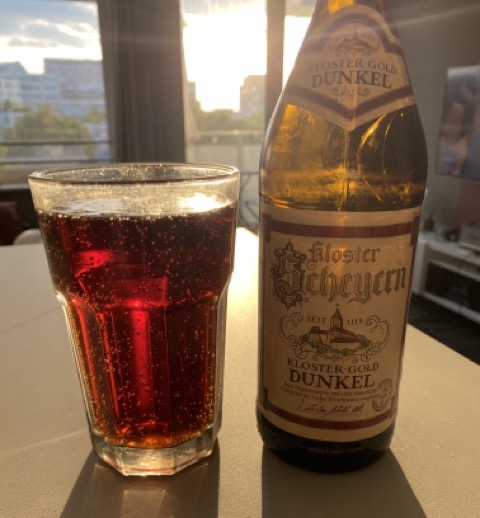
\includegraphics[height=3.2cm]{img/beer3.jpeg}}\\
        \vfill
        \onslide<7->{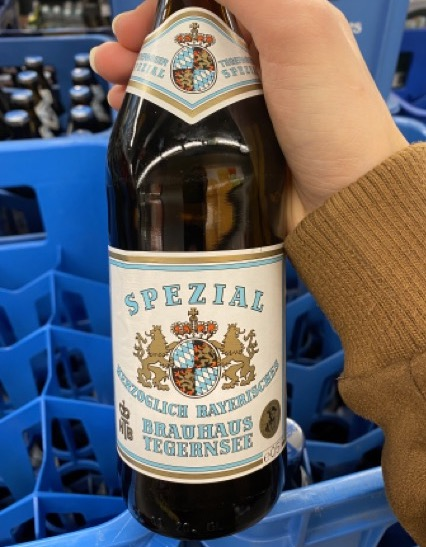
\includegraphics[height=3.2cm]{img/beer4.jpeg}}
        \onslide<8->{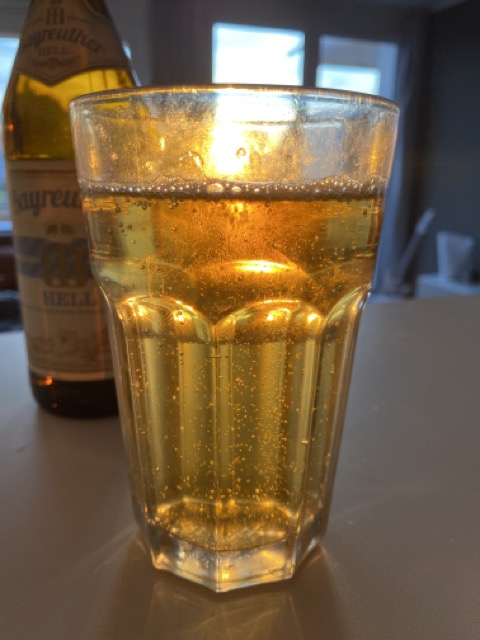
\includegraphics[height=3.2cm]{img/beer5.jpeg}}
        \onslide<9->{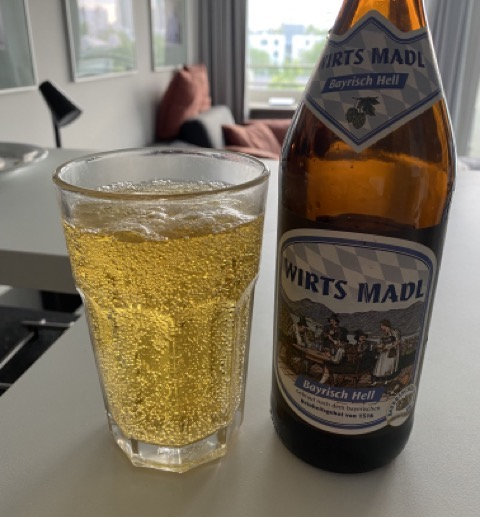
\includegraphics[height=3.2cm]{img/beer6.jpeg}}
        \onslide<10->{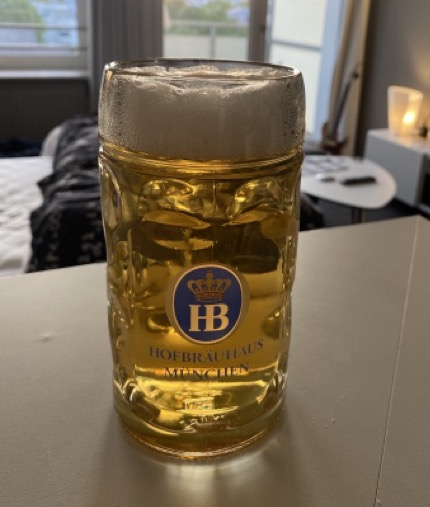
\includegraphics[height=3.2cm]{img/beer7.jpeg}}
    \end{figure}
    }
\end{frame}

\subsection{Technical University of Munich}

\begin{frame}
    \begin{figure}
        \begin{subfigure}{0.3\textwidth}
            \centering
            
\includegraphics[height=1cm]{../img/logoTUM.png}\\
            \vspace*{1cm}
            
\includegraphics[height=1.5cm]{../img/logoisabelle.png}
        \end{subfigure}
        \begin{subfigure}{0.69\textwidth}
            \centering
            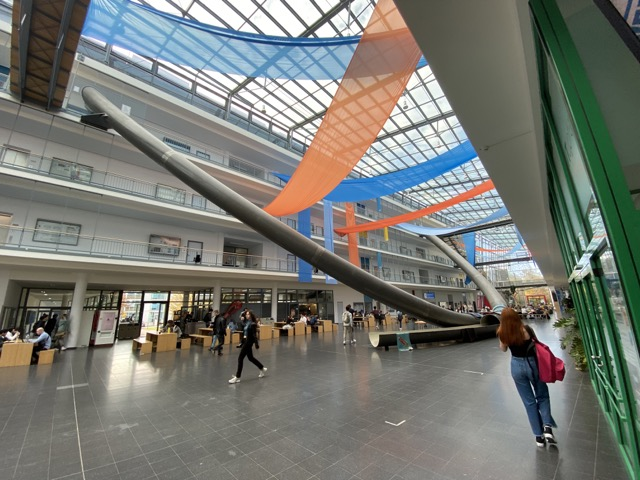
\includegraphics[height=6cm]{img/TUM.jpeg}
        \end{subfigure}
        \caption{Technical University of Munich (TUM)}
    \end{figure}
\end{frame}


\end{document}